%%%%%%%%%%%%%%%%%%%%%%%%%%%%%%%%%%%%%%%%%%%%%%%%%%%%%%%%%%%%%%%%%%%%%%%%%%%%%%
% CHAPTER 7
% CONCLUSION & FUTURE DEVELOPMENT
%%%%%%%%%%%%%%%%%%%%%%%%%%%%%%%%%%%%%%%%%%%%%%%%%%%%%%%%%%%%%%%%%%%%%%%%%%%%%%

\chapter{CONCLUSION \& FUTURE DEVELOPMENT}

\section{Giới thiệu chương}

Chương này trình bày tổng kết về quá trình thực hiện đồ án môn học "Hệ thống quản lý cuộc thi SEAL Hackathon" và đánh giá kết quả đạt được so với các mục tiêu đã đề ra ban đầu. Đồng thời, chương cũng đề xuất các hướng phát triển trong tương lai nhằm hoàn thiện và mở rộng hệ thống để đáp ứng tốt hơn nhu cầu thực tế của các cuộc thi Hackathon trong ngành Kỹ thuật Phần mềm.

Quá trình phát triển hệ thống SEAL Hackathon Management System đã trải qua các giai đoạn từ phân tích yêu cầu, thiết kế hệ thống, hiện thực hóa các chức năng cho đến kiểm thử và đánh giá chất lượng. Mỗi giai đoạn đều được nhóm thực hiện một cách nghiêm túc, có kế hoạch và tuân thủ theo quy trình phát triển phần mềm Agile Scrum.

Các nội dung chính được trình bày trong chương bao gồm: tổng kết các công việc đã hoàn thành, đánh giá mức độ đáp ứng các yêu cầu chức năng và phi chức năng, phân tích những hạn chế còn tồn tại của hệ thống hiện tại, và đề xuất các giải pháp phát triển trong tương lai.

\section{Hình ảnh minh họa hệ thống}

Để minh họa cho các chức năng đã được hiện thực hóa, báo cáo này chèn một số hình ảnh trực quan từ hệ thống như sau:

\begin{figure}[H]
\centering
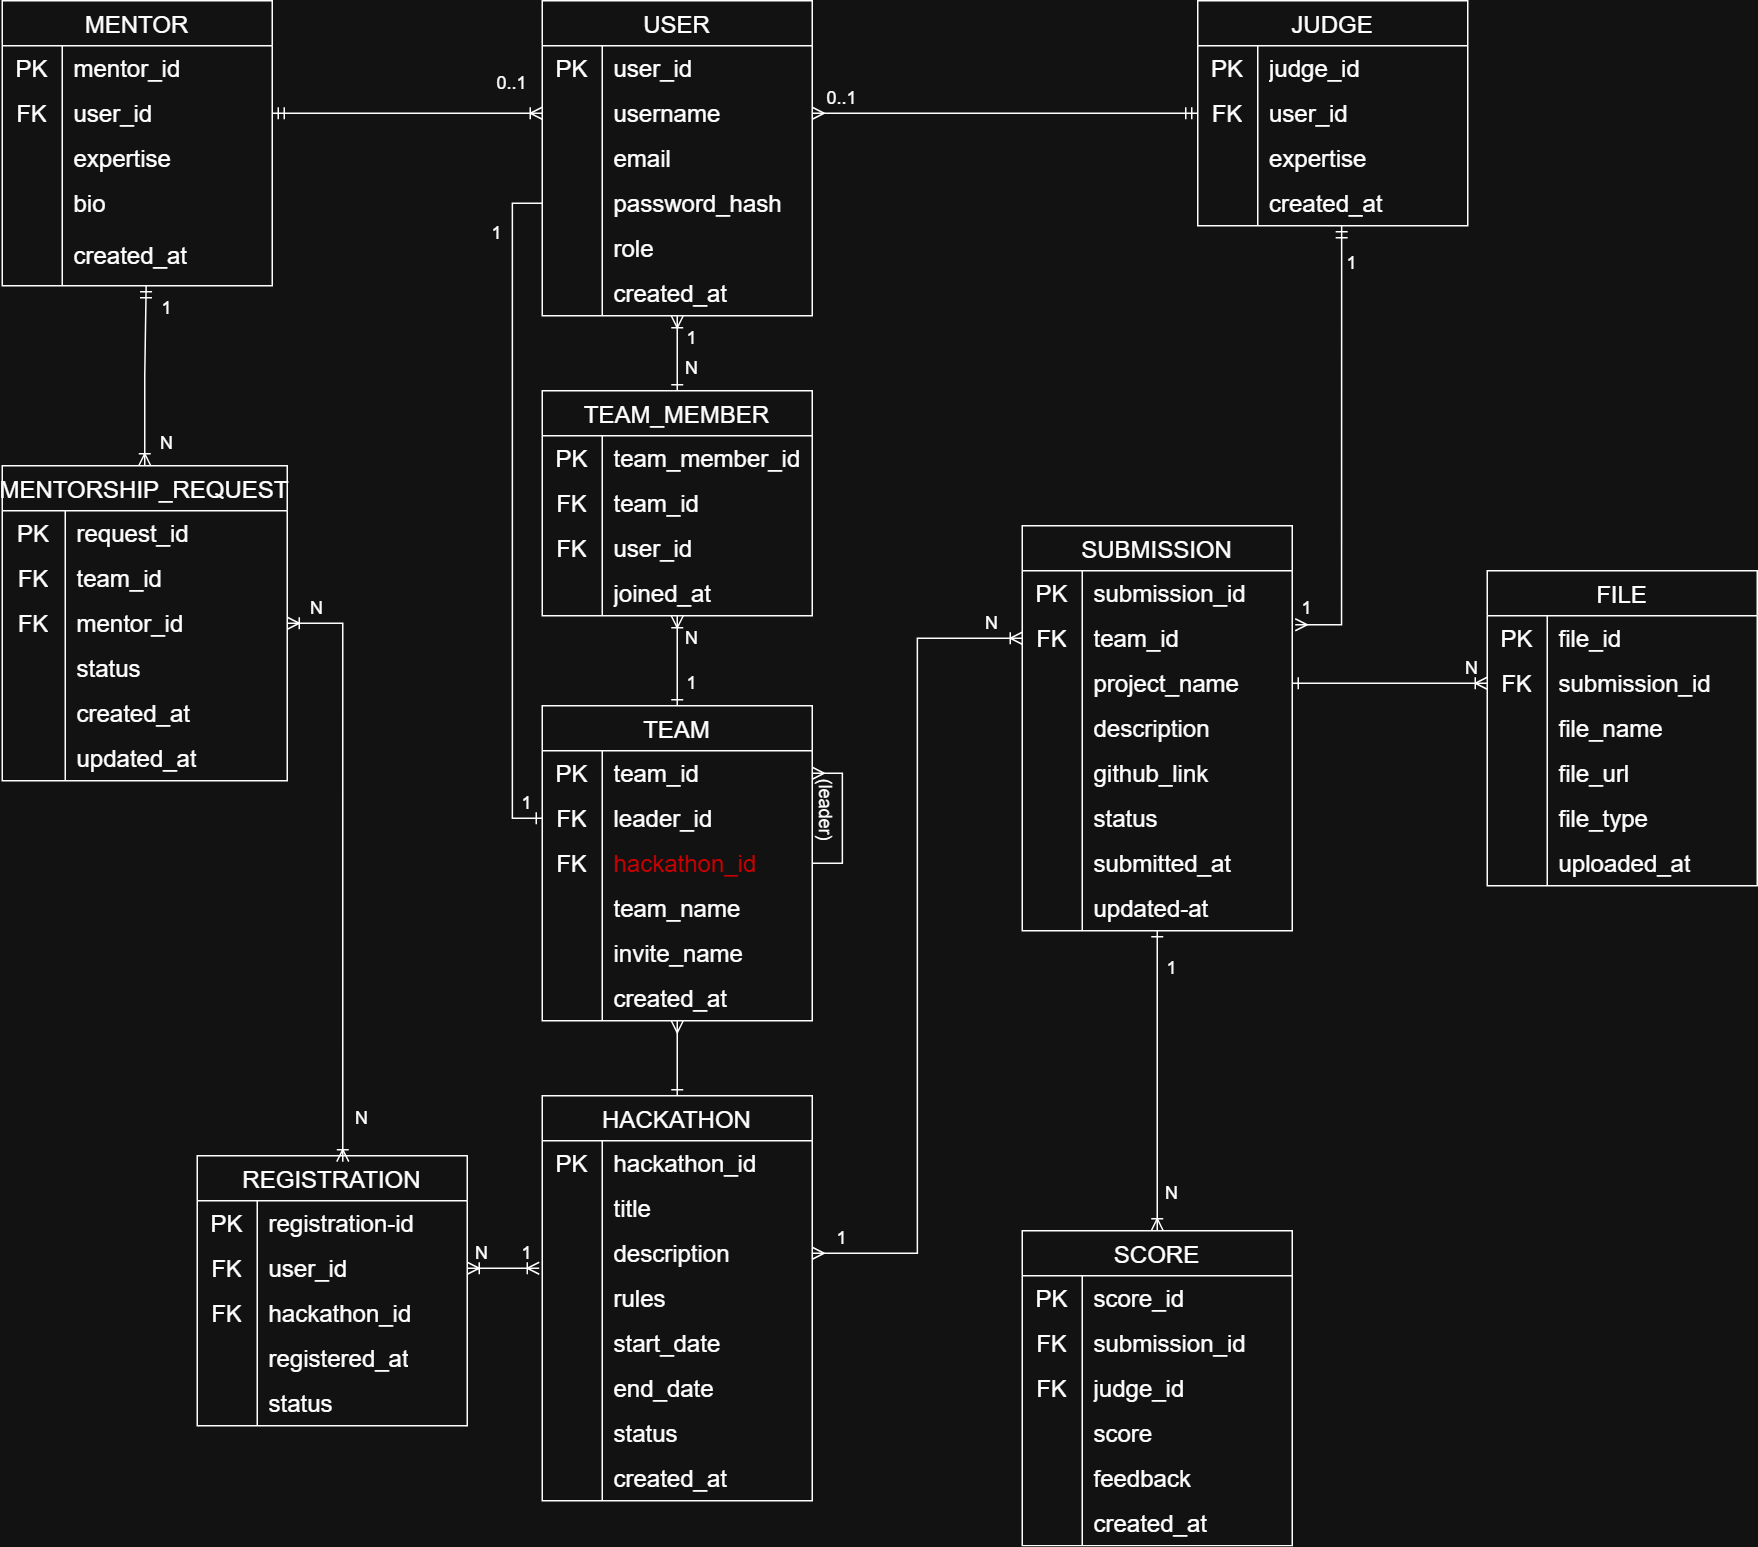
\includegraphics[width=0.9\textwidth]{ERD.png}
\caption{Mô hình ERD của hệ thống SEAL Hackathon Management}
\label{fig:erd}
\end{figure}

\begin{figure}[H]
\centering

\includegraphics[width=0.9\textwidth]{dashboard_team_info.png}
\caption{Giao diện Dashboard hiển thị thông tin đội thi}
\label{fig:dashboard}
\end{figure}

%%%%%%%%%%%%%%%%%%%%%%%%%%%%%%%%%%%%%%%%%%%%%%%%%%%%%%%%%%%%%%%%%%%%%%%%%%%%%%

\section{Tổng kết công việc đã hoàn thành}

\subsection{Các mục tiêu đã đạt được}

Sau quá trình phát triển và kiểm thử, hệ thống SEAL Hackathon Management System đã đạt được các mục tiêu quan trọng sau:

\begin{itemize}
	\item \textbf{Hoàn thành hệ thống quản lý cuộc thi Hackathon đầy đủ chức năng cơ bản:} Hệ thống cho phép người dùng đăng ký tài khoản, đăng nhập, tạo đội thi, quản lý thành viên, nộp bài dự thi và quản lý các thông tin liên quan đến cuộc thi một cách hiệu quả.
	
	\item \textbf{Áp dụng kiến trúc RESTful API hiện đại:} Backend được xây dựng bằng FastAPI với kiến trúc RESTful, cho phép giao tiếp linh hoạt với Frontend thông qua định dạng JSON, đảm bảo tính mở rộng và dễ bảo trì.
	
	\item \textbf{Triển khai cơ chế xác thực và phân quyền người dùng:} Hệ thống sử dụng JWT Authentication để bảo mật các API endpoint, đồng thời phân quyền rõ ràng giữa Trưởng đội và Thành viên trong quá trình quản lý đội.
	
	\item \textbf{Xây dựng giao diện người dùng trực quan và dễ sử dụng:} Frontend được thiết kế với HTML5, CSS3 và JavaScript thuần, cung cấp giao diện Dashboard thân thiện, giúp người dùng dễ dàng thực hiện các thao tác cần thiết.
	
	\item \textbf{Kiểm thử toàn diện các chức năng chính:} Hệ thống đã được kiểm thử qua 16 trường hợp kiểm thử bao phủ các chức năng quan trọng như đăng ký, đăng nhập, quản lý đội, quản lý thành viên và nộp bài. Kết quả kiểm thử cho thấy toàn bộ các chức năng đều hoạt động ổn định và đúng theo yêu cầu.
	
	\item \textbf{Lưu trữ dữ liệu an toàn với cơ sở dữ liệu SQLite:} Hệ thống sử dụng SQLite kết hợp với SQLAlchemy ORM để quản lý dữ liệu, đảm bảo tính toàn vẹn và nhất quán của thông tin người dùng, đội thi và bài nộp.
	
	\item \textbf{Phát triển theo quy trình Agile Scrum:} Nhóm áp dụng phương pháp Agile Scrum với các Sprint định kỳ, sử dụng Jira để quản lý task và theo dõi tiến độ, giúp đảm bảo dự án hoàn thành đúng hạn.
	
	\item \textbf{Tài liệu hóa đầy đủ hệ thống:} Các tài liệu kỹ thuật bao gồm SRS (Software Requirements Specification), SDD (Software Design Description) và tài liệu kiểm thử được xây dựng chi tiết, tạo cơ sở cho việc bảo trì và phát triển tiếp theo.
\end{itemize}

%%%%%%%%%%%%%%%%%%%%%%%%%%%%%%%%%%%%%%%%%%%%%%%%%%%%%%%%%%%%%%%%%%%%%%%%%%%%%%

\subsection{Các chức năng đã hiện thực hóa}

Hệ thống SEAL Hackathon Management System đã hiện thực hóa thành công các nhóm chức năng chính sau:

\begin{table}[H]
	\centering
	\caption{Tổng hợp các chức năng đã hoàn thành}
	\label{tab:completed-features}
	\renewcommand{\arraystretch}{1.3}
	\begin{tabular}{|p{4cm}|p{10cm}|}
		\hline
		\textbf{Nhóm chức năng} & \textbf{Các chức năng đã hoàn thành} \\
		\hline
		Quản lý tài khoản & Đăng ký tài khoản, đăng nhập, đăng xuất, xác thực JWT \\
		\hline
		Quản lý đội thi & Tạo đội, sinh mã mời, giải tán đội, hiển thị thông tin đội \\
		\hline
		Quản lý thành viên & Tham gia đội, phê duyệt thành viên, kick thành viên, rời đội \\
		\hline
		Quản lý bài nộp & Nộp đường dẫn GitHub, cập nhật bài nộp, hiển thị trạng thái \\
		\hline
		Giao diện người dùng & Dashboard theo vai trò, thông báo lỗi, điều hướng chức năng \\
		\hline
	\end{tabular}
\end{table}

Các chức năng trên đã được kiểm thử và vận hành ổn định, đáp ứng đủ nhu cầu cơ bản của một cuộc thi Hackathon quy mô nhỏ và trung bình.

%%%%%%%%%%%%%%%%%%%%%%%%%%%%%%%%%%%%%%%%%%%%%%%%%%%%%%%%%%%%%%%%%%%%%%%%%%%%%%

\section{Đánh giá mức độ đáp ứng yêu cầu}

\subsection{Đánh giá yêu cầu chức năng}

Hệ thống đã đáp ứng thành công các yêu cầu chức năng cốt lõi được đặc tả trong tài liệu Software Requirements Specification (SRS):

\begin{itemize}
	\item \textbf{Quản lý người dùng:} Hệ thống cho phép đăng ký tài khoản mới với kiểm tra tính duy nhất của Username và Email. Chức năng đăng nhập sử dụng JWT Token để bảo mật phiên làm việc.
	
	\item \textbf{Quản lý đội thi:} Người dùng có thể tạo đội mới với tên đội tự định nghĩa, hệ thống tự động sinh mã mời gồm 6 ký tự để chia sẻ với thành viên khác. Chức năng giải tán đội chỉ được thực hiện bởi Trưởng đội.
	
	\item \textbf{Quản lý thành viên:} Thành viên có thể gửi yêu cầu tham gia đội thông qua mã mời. Trưởng đội có quyền phê duyệt hoặc từ chối yêu cầu, đồng thời có thể loại thành viên khỏi đội khi cần thiết.
	
	\item \textbf{Quản lý bài nộp:} Trưởng đội có thể nộp đường dẫn GitHub của dự án và cập nhật lại đường dẫn khi cần thiết. Hệ thống lưu trữ thông tin bài nộp để phục vụ quá trình đánh giá.
	
	\item \textbf{Phân quyền người dùng:} Hệ thống phân quyền rõ ràng giữa Trưởng đội và Thành viên, đảm bảo mỗi người dùng chỉ được thực hiện các thao tác trong quyền hạn của mình.
\end{itemize}

Tuy nhiên, một số yêu cầu chức năng nâng cao như hệ thống chấm điểm tự động, quản lý Mentor, quản lý vòng thi và xuất báo cáo chi tiết chưa được hiện thực hóa trong phiên bản hiện tại do giới hạn về thời gian và phạm vi của đồ án môn học.

%%%%%%%%%%%%%%%%%%%%%%%%%%%%%%%%%%%%%%%%%%%%%%%%%%%%%%%%%%%%%%%%%%%%%%%%%%%%%%

\subsection{Đánh giá yêu cầu phi chức năng}

\begin{itemize}
	\item \textbf{Tính sử dụng (Usability):} Giao diện Dashboard được thiết kế đơn giản, trực quan với các chức năng được phân nhóm rõ ràng. Người dùng có thể dễ dàng thực hiện các thao tác mà không cần hướng dẫn chi tiết.
	
	\item \textbf{Tính tin cậy (Reliability):} Hệ thống hoạt động ổn định trong quá trình kiểm thử, dữ liệu được lưu trữ chính xác trong cơ sở dữ liệu SQLite và được đồng bộ hóa giữa Frontend và Backend.
	
	\item \textbf{Tính hiệu năng (Performance):} Hệ thống phản hồi nhanh đối với các thao tác cơ bản như đăng nhập, tạo đội, nộp bài. Tuy nhiên, chưa được kiểm thử với số lượng lớn người dùng truy cập đồng thời.
	
	\item \textbf{Tính bảo mật (Security):} Mật khẩu được mã hóa bằng BCrypt trước khi lưu vào cơ sở dữ liệu. JWT Authentication được sử dụng để bảo vệ các API endpoint. Tuy nhiên, hệ thống chưa triển khai các biện pháp bảo mật chuyên sâu như CSRF protection, rate limiting hay encryption cho dữ liệu nhạy cảm.
	
	\item \textbf{Tính khả năng bảo trì (Maintainability):} Mã nguồn được viết theo cấu trúc rõ ràng, có comment và tuân thủ các quy tắc coding convention. Các tài liệu kỹ thuật được xây dựng đầy đủ hỗ trợ quá trình bảo trì.
	
	\item \textbf{Tính khả năng mở rộng (Scalability):} Kiến trúc RESTful API và việc sử dụng ORM giúp hệ thống có khả năng mở rộng. Tuy nhiên, việc sử dụng SQLite có thể hạn chế khả năng mở rộng khi dữ liệu tăng lên lớn.
\end{itemize}

%%%%%%%%%%%%%%%%%%%%%%%%%%%%%%%%%%%%%%%%%%%%%%%%%%%%%%%%%%%%%%%%%%%%%%%%%%%%%%

\section{Những hạn chế và khó khăn gặp phải}

\subsection{Hạn chế về phạm vi chức năng}

Do giới hạn về thời gian và nguồn lực của đồ án môn học, hệ thống hiện tại chưa bao gồm một số chức năng quan trọng:

\begin{itemize}
	\item Chưa có hệ thống chấm điểm tự động cho giám khảo.
	\item Chưa có chức năng quản lý Mentor và theo dõi đội thi.
	\item Chưa có chức năng quản lý vòng thi và hạng mục thi.
	\item Chưa có chức năng xuất báo cáo và thống kê kết quả.
	\item Chưa có hệ thống thông báo thời gian thực (real-time notification).
	\item Chưa có chức năng quản lý file và tài liệu đính kèm.
\end{itemize}

%%%%%%%%%%%%%%%%%%%%%%%%%%%%%%%%%%%%%%%%%%%%%%%%%%%%%%%%%%%%%%%%%%%%%%%%%%%%%%

\subsection{Hạn chế về kỹ thuật}

\begin{itemize}
	\item Sử dụng SQLite làm cơ sở dữ liệu có thể không phù hợp khi hệ thống mở rộng với lượng dữ liệu lớn và nhiều người dùng truy cập đồng thời.
	\item Frontend sử dụng JavaScript thuần chưa áp dụng các framework hiện đại như React hay Vue.js, làm giảm khả năng tái sử dụng component và quản lý state phức tạp.
	\item Hệ thống chưa được triển khai trên môi trường Cloud, chỉ chạy cục bộ trên máy phát triển.
	\item Chưa có hệ thống CI/CD tự động cho quá trình deploy và kiểm thử.
	\item Chưa có hệ thống logging và monitoring chuyên sâu để theo dõi trạng thái hệ thống trong môi trường production.
\end{itemize}

%%%%%%%%%%%%%%%%%%%%%%%%%%%%%%%%%%%%%%%%%%%%%%%%%%%%%%%%%%%%%%%%%%%%%%%%%%%%%%

\subsection{Khó khăn trong quá trình phát triển}

\begin{itemize}
	\item \textbf{Đồng bộ hóa giữa Frontend và Backend:} Trong giai đoạn đầu, nhóm gặp khó khăn trong việc đảm bảo dữ liệu được đồng bộ chính xác giữa giao diện người dùng và cơ sở dữ liệu sau mỗi thao tác.
	
	\item \textbf{Quản lý state trong Frontend:} Việc sử dụng JavaScript thuần để quản lý trạng thái của Dashboard gặp khó khăn khi số lượng chức năng tăng lên, dẫn đến cần phải reload dữ liệu nhiều lần.
	
	\item \textbf{Xử lý lỗi ngoại lệ:} Một số lỗi như đăng xuất không hoạt động, Dashboard hiển thị dữ liệu mẫu đã phát sinh và cần thời gian để debug và khắc phục.
	
	\item \textbf{Thiết kế API:} Việc thiết kế RESTful API cần đảm bảo tính nhất quán và tuân thủ các chuẩn REST đòi hỏi sự cân nhắc kỹ lưỡng về cấu trúc dữ liệu request và response.
\end{itemize}

Mặc dù gặp những khó khăn trên, nhóm đã từng bước giải quyết thông qua quá trình kiểm thử, debug và cải tiến mã nguồn, đảm bảo hệ thống hoạt động ổn định trước khi hoàn thiện.

%%%%%%%%%%%%%%%%%%%%%%%%%%%%%%%%%%%%%%%%%%%%%%%%%%%%%%%%%%%%%%%%%%%%%%%%%%%%%%

\section{Hướng phát triển trong tương lai}

\subsection{Mở rộng chức năng quản lý cuộc thi}

Trong các phiên bản tiếp theo, hệ thống có thể được mở rộng với các chức năng quản lý cuộc thi chuyên sâu hơn:

\begin{itemize}
	\item \textbf{Quản lý vòng thi:} Cho phép Ban tổ chức tạo và quản lý nhiều vòng thi khác nhau (Vòng loại, Vòng bán kết, Vòng chung kết) với thời gian và quy tắc riêng.
	
	\item \textbf{Quản lý hạng mục thi:} Hỗ trợ đa dạng hạng mục thi như Web Application, Mobile Application, AI/ML, IoT, v.v.
	
	\item \textbf{Hệ thống chấm điểm tự động:} Xây dựng module chấm điểm cho Giám khảo với các tiêu chí đánh giá có thể tùy chỉnh, tính điểm tự động và xếp hạng đội thi.
	
	\item \textbf{Quản lý Mentor:} Cho phép Mentor theo dõi tiến độ của các đội, gửi góp ý và đánh giá quá trình phát triển dự án.
	
	\item \textbf{Xuất báo cáo:} Cung cấp chức năng xuất báo cáo thống kê về số lượng đội, kết quả chấm điểm, biểu đồ xếp hạng và các chỉ số liên quan.
\end{itemize}

%%%%%%%%%%%%%%%%%%%%%%%%%%%%%%%%%%%%%%%%%%%%%%%%%%%%%%%%%%%%%%%%%%%%%%%%%%%%%%

\subsection{Cải thiện kỹ thuật và kiến trúc}

\begin{itemize}
	\item \textbf{Chuyển đổi sang PostgreSQL hoặc MySQL:} Thay thế SQLite bằng hệ quản trị cơ sở dữ liệu mạnh mẽ hơn để hỗ trợ lượng dữ liệu lớn và nhiều người dùng truy cập đồng thời.
	
	\item \textbf{Áp dụng Frontend Framework:} Sử dụng React.js hoặc Vue.js để xây dựng Frontend, giúp quản lý state tốt hơn, tái sử dụng component và cải thiện trải nghiệm người dùng.
	
	\item \textbf{Triển khai trên Cloud:} Đưa hệ thống lên các nền tảng Cloud như AWS, Google Cloud hoặc Azure để đảm bảo tính sẵn sàng cao và khả năng mở rộng tự động.
	
	\item \textbf{Thêm hệ thống Cache:} Sử dụng Redis để cache dữ liệu thường xuyên truy cập, giúp giảm tải cho cơ sở dữ liệu và cải thiện hiệu năng.
	
	\item \textbf{Triển khai CI/CD:} Xây dựng pipeline CI/CD với GitHub Actions hoặc GitLab CI để tự động hóa quá trình kiểm thử và deploy.
	
	\item \textbf{Thêm hệ thống Logging và Monitoring:} Sử dụng các công cụ như ELK Stack (Elasticsearch, Logstash, Kibana) hoặc Prometheus + Grafana để theo dõi trạng thái hệ thống và phát hiện lỗi sớm.
\end{itemize}

%%%%%%%%%%%%%%%%%%%%%%%%%%%%%%%%%%%%%%%%%%%%%%%%%%%%%%%%%%%%%%%%%%%%%%%%%%%%%%

\subsection{Nâng cao tính bảo mật}

\begin{itemize}
	\item \textbf{Thêm Rate Limiting:} Giới hạn số lượng request từ một IP trong khoảng thời gian nhất định để ngăn chặn DDoS attack.
	
	\item \textbf{CSRF Protection:} Triển khai cơ chế bảo vệ CSRF để ngăn chặn các tấn công giả mạo request từ người dùng đã xác thực.
	
	\item \textbf{Input Validation nâng cao:} Kiểm tra và làm sạch dữ liệu đầu vào nghiêm ngặt hơn để ngăn chặn các tấn công như XSS, SQL Injection.
	
	\item \textbf{HTTPS:} Triển khai SSL/TLS để mã hóa toàn bộ traffic giữa client và server.
	
	\item \textbf{Audit Log chi tiết:} Ghi nhật ký chi tiết cho mọi thao tác quan trọng của người dùng để phục vụ mục đích audit và forensic.
\end{itemize}

%%%%%%%%%%%%%%%%%%%%%%%%%%%%%%%%%%%%%%%%%%%%%%%%%%%%%%%%%%%%%%%%%%%%%%%%%%%%%%

\subsection{Cải thiện trải nghiệm người dùng}

\begin{itemize}
	\item \textbf{Real-time Notification:} Triển khai WebSocket để gửi thông báo thời gian thực cho người dùng về các sự kiện như có thành viên mới tham gia đội, bài nộp được chấm điểm, v.v.
	
	\item \textbf{Mobile Application:} Phát triển ứng dụng di động (iOS/Android) để người dùng có thể truy cập hệ thống từ mọi thiết bị.
	
	\item \textbf{Giao diện đa ngôn ngữ:} Hỗ trợ đa ngôn ngữ (Tiếng Việt, Tiếng Anh) để mở rộng đối tượng người dùng.
	
	\item \textbf{Dark Mode:} Thêm chế độ giao diện tối để cải thiện trải nghiệm người dùng trong môi trường ánh sáng yếu.
	
	\item \textbf{Trợ lý ảo:} Tích hợp chatbot AI để hỗ trợ người dùng giải đáp các câu hỏi thường gặp và hướng dẫn sử dụng hệ thống.
\end{itemize}

%%%%%%%%%%%%%%%%%%%%%%%%%%%%%%%%%%%%%%%%%%%%%%%%%%%%%%%%%%%%%%%%%%%%%%%%%%%%%%

\section{Bài học kinh nghiệm}

Quá trình thực hiện đồ án "Hệ thống quản lý cuộc thi SEAL Hackathon" đã mang lại cho nhóm nhiều bài học kinh nghiệm quý báu:

\begin{itemize}
	\item \textbf{Kỹ năng làm việc nhóm:} Việc phối hợp giữa 7 thành viên với các vai trò khác nhau đòi hỏi kỹ năng giao tiếp, phân chia công việc và trách nhiệm cao. Agile Scrum đã giúp nhóm quản lý tiến độ hiệu quả.
	
	\item \textbf{Quy trình phát triển phần mềm:} Nhóm đã học được tầm quan trọng của việc tuân thủ quy trình từ phân tích yêu cầu, thiết kế, hiện thực đến kiểm thử. Mỗi giai đoạn đều đóng vai trò quan trọng trong chất lượng sản phẩm cuối cùng.
	
	\item \textbf{Kiến thức kỹ thuật:} Việc áp dụng FastAPI, JWT Authentication, SQLAlchemy và các công nghệ hiện đại khác đã giúp nhóm mở rộng kiến thức về phát triển Backend và kiến trúc RESTful API.
	
	\item \textbf{Kỹ năng giải quyết vấn đề:} Quá trình debug và khắc phục các lỗi đã giúp nhóm rèn luyện tư duy logic và kỹ năng phân tích vấn đề một cách hệ thống.
	
	\item \textbf{Tài liệu hóa:} Việc xây dựng tài liệu kỹ thuật chi tiết không chỉ hỗ trợ quá trình phát triển mà còn tạo giá trị cho việc bảo trì và chuyển giao dự án.
	
	\item \textbf{Quản lý thời gian:} Làm việc với deadline và các Sprint định kỳ giúp nhóm rèn luyện kỹ năng quản lý thời gian và ưu tiên công việc.
\end{itemize}

Những bài học này sẽ là nền tảng quan trọng cho nhóm trong các dự án phần mềm trong tương lai.

%%%%%%%%%%%%%%%%%%%%%%%%%%%%%%%%%%%%%%%%%%%%%%%%%%%%%%%%%%%%%%%%%%%%%%%%%%%%%%

\section{Kết luận}

Hệ thống quản lý cuộc thi SEAL Hackathon đã được phát triển thành công với đầy đủ các chức năng cơ bản cần thiết để quản lý một cuộc thi Hackathon quy mô nhỏ và trung bình. Hệ thống đáp ứng tốt các yêu cầu về quản lý tài khoản, quản lý đội thi, quản lý thành viên và nộp bài dự thi, đồng thời đảm bảo tính bảo mật và trải nghiệm người dùng ở mức độ chấp nhận được.

Quá trình kiểm thử cho thấy toàn bộ 16 trường hợp kiểm thử đều đạt trạng thái PASS, chứng minh các chức năng hoạt động ổn định và đúng theo yêu cầu thiết kế. Các lỗi phát hiện trong quá trình phát triển đều đã được khắc phục và kiểm thử lại.

Mặc dù hệ thống còn một số hạn chế về phạm vi chức năng và kỹ thuật, nhưng đây là nền tảng vững chắc để tiếp tục phát triển trong tương lai. Các hướng phát triển đã đề xuất như mở rộng chức năng quản lý cuộc thi, cải thiện kiến trúc kỹ thuật, nâng cao tính bảo mật và cải thiện trải nghiệm người dùng sẽ giúp hệ thống trở nên hoàn thiện hơn và đáp ứng tốt hơn nhu cầu thực tế.

Đồ án này không chỉ là kết quả của quá trình học tập mà còn là cơ hội để nhóm rèn luyện các kỹ năng thực tế trong phát triển phần mềm, làm việc nhóm và quản lý dự án. Nhóm hy vọng rằng hệ thống sẽ được tiếp tục phát triển và ứng dụng thực tế trong các cuộc thi Hackathon của ngành Kỹ thuật Phần mềm.

